% Intro - luźne przemyślenia
%- Chcemy aby każdy członek zespołu stosował podobne zasady, wzorce i nazewnictwo. 
%- Wzorce i struktura są często dużo ważniejsze niż same algorytmy. 
%- Zazwyczaj temat wzorców projektowych, zasad SOLID, TDD czy refaktoringu pojawia się podczas rozmów kwalifikacyjnych. 
%- Wzorce i wspominane zasady SOLILD pozwalają odpowiedziec na pytanie jak podzielić projekt na niezależne komponenty, tak aby można było łatwo je rozszerzać i zamieniać, bez konieczności wprowadzania zmian w pozostałych komponentach. Dobry podział pozwala na szybsze znajdowanie błędów w oprogramowaniu. Jeżeli przepływ informacji jest prosty nie powinno być ciężko dowiedzieć się czy błąd znajduje się w warstwie logiki biznesowej, w kontrolerze czy widoku.
%- Z wzorcem Singleton może istnieć problem, że mamy dwa takie obiekty, które ze sobą rozmawiają. Przepływ informacji jest dwukierunkowy, który sprawia, że ciężej jest zrozumieć program i go debugować. Zazwyczaj zależy nam na jednokierunkowym przepływie informacji.
%- Obiekty modelu powinny zawierać jedynie takie zachowania, które bezpośrednio zmieniają ich stan. Nie powinny one zawierać logiki biznesowej.

\section{Zasady SOLID}

W publikacji \texttt{Design Principles and Design Patterns} Robert C. Martin opisał 5 zasad SOLID, które pomagają uzyskać lepszy, bardziej zrozumiały i łatwiejszy w utrzymaniu oraz rozbudowie kod. Są one również trzonem metodologi takich jak Agile czy programowanie adaptywne. W kolejnych podrozdziałach zostaną one po kolei opisane. 

\subsection{SRP - Zasada pojedynczej odpowiedzialności (ang. \textbf{S}OLID)}\label{lab1/sec/srpPrinciple}

Pierwsza z pięciu zasad mówi, że każdy moduł, zestaw, klasa czy metoda powinna posiadać pojedynczy obszar odpowiedzialności (przyczynę zmian).  W momencie zmian wymagań, określa się jakie klasy są odpowiedzialne za dane wymagania i to te kasy się modyfikuje. Jeśli istnieją co najmniej dwa niezależne powody mogące wymusić zmianę w danej klasie, to dana klasa rozciąga się na więcej niż jeden obszar odpowiedzialności. W~przypadku naruszenia zasady SRP zmiany w dwóch różnych wymaganiach implikują modyfikację w jednej, tej samej klasie. 
%Niepożądane są tzw. ,,boskie klasy'' (ang. God classes), które są odpowiedzialne za wiele rzeczy. 

\begin{myboxWithTitle}{Zasada pojedynczej odpowiedzialności}
	Żadna klasa nie może być modyfikowana z więcej niż jednego powodu.
\end{myboxWithTitle}

Wyobraźmy sobie sytuację, w której klasa rysująca na ekranie figurę geometryczną np. \texttt{Rectangle} jest odpowiedzialna zarówno za wspomniane rysowanie, ale również za wyznaczanie pola powierzchni danej figury. Jakie konsekwencje to za sobą niesie? Jeśli dwa zestawy np. interfejsu użytkownika \texttt{UI} oraz jakiś inny korzystający jedynie z operacji liczenia pola powierzchni będą związane z klasą \texttt{Rectangle} to zmiana wynikająca z wymagań związanych z \texttt{UI} może pociągać ryzyko nieprawidłowego działania w drugim zestawie. Aby nie naruszyć zasady SRP należałoby stworzyć dwie osobne klasy: jedną rysująca figurę i drugą liczącą pole powierzchni. Pierwsza z~nich mogłaby wykorzystywać tę pierwszą. 

Oczywiście należy zawsze mieć na uwadze, że rozdrabniać klasy na coraz mniejsze typy można prawie w~nieskończoność. Może to prowadzić do nadmiernego skomplikowania projektu. Konieczne jest branie pod uwagę wymagań i ich potencjalnych zmian.

Jako przykład przeanalizujmy interfejs \texttt{IModem}.
\begin{lstlisting}[caption={Naruszenie zasady SRP}, label={lab1/lst/srpViolationModem}]
	public interface IModem
	{
		public void Dial(string phoneNumber);
		public void Hangup();
		public void Send(char c);
		public char Recieve();
	}
\end{lstlisting}
Widać, że interfejs mógłby zostać podzielony na dwa obszary odpowiedzialności. Jeden odpowiadający za nawiązywanie i zrywanie połączeń, drugi natomiast za same funkcje komunikacyjne. Klasy klienckie mogłyby wykorzystywać klasę implementującą dwa interfejsy np. \texttt{IDataChannel} i \texttt{IConnection} i tym samym uzależnić się tylko od jednego z obszarów odpowiedzialności. 
%Tutaj konieczne jest przeanalizowanie wymagań, ponieważ podział interfejsu na dwa zawierające odpowiednio \texttt{Dial} i \texttt{Hangup} oraz \texttt{Send} i \texttt{Recieve} może nie być potrzebny, jeśli zmiany w aplikacji nie wpływają na zmiany w~metodach zarządzających wykonywaniem połączeń.
% [DataChannel]^-.-[ModemImplementation]
% [Connection]^-.-[ModemImplementation]
%[<<interface>>;DataChannel|+send(c:char);+recv():char]
%[<<interface>>;Connection|+dial(pno: String);+hangup()]

%\subsubsection{Zadanie 1}
%\begin{lstlisting}[caption={Naruszenie zasady SRP}, label={lab1/lst/srpViolationEmployee}]
%class Employee()
%{
%	public void CalculatePay();
%	public void ReportHours();
%	public void Store();
%}
%\end{lstlisting}
%W powyższym przykładzie została naruszona zasada SRP, zaproponuj sposób rozdzielenia odpowiedzialności tej klasy. 
%
%Utwórz nowy projekt .NET 5.0 i dodaj do niego klasy, które pozwolą na implementację zachowań klasy \texttt{Employee} tak, aby zachować zasadę SRP.

% Zakładamy, że te trzy metody są wykorzystywane przez innego aktora. Np. CalculatePay przez dział księgowości, ReportHours przez dział kadr, a Store() przez dział administrowania bazami danych. Umieszczając to w jednej klasie zostały połączone odpowiedzialności trzech aktórów. 
% Dodatkowo złączenia (merge) w gitcie są dość ryzykowne, a dzieje się tak często jeśli dwóch programistów pracuje nad tą samą klasą.


% Podejść do problemu można na trzy sposoby:
% 1. Trzy osobne klasy, PayCalculator, HourReporter oraz EmployeeSaver, które współdzielą dostęp do klasy EmployeeData (struktura danych)
% 2. Rozwinięcie punktu nr 1. Zastosować wzorzec Fasada, która tworzy i deleguje zadania wywołania do odpowiednich klas i ich funkcji. Pozwala to uniknąć problemu, konieczności tworzenia i żąglowania trzema obiektami. 
% 3. Utrzymać reguły biznesowe blisko właściwych danych. Klasa Employee może stać fasadą dla pomniejszych funkcji. Może zawierać klasy (lepiej referencje do interfejsów) do HourReporter i EmployeeSaver. Sama natomiast może posiadać employeeData, CalculatePay(), ReportHours(), Store() - te dwie ostatnie mogłyby delegować zadania do odpowiednich implementacji przekazanych np. jako argumenty konstruktora. 

% Reguły biznesowe jak i mechanizmy wiedzialności nigdy nie powinny być ze sobą łączone. Powodu do ich zmian są różne. 
% Możemy powyższą klasę podzielić na trzy mniejsze klasy:
%\begin{itemize}
%	\item PayCalculator z metodą CalculatePay,
%	\item HourReporter z metodą ReportHours,
%	\item EmployeeRepository z metodą SaveEmployee.
%\end{itemize}
%Każda z tych klas może korzystać z encji \texttt{EmployeeData}.



\subsubsection{Zadanie 1}

Poniżej przedstawiony fragment kodu\cite{adaptatywny_kod_hall} zawiera klasę\ref{lab1/lst/srpViolationEmployee} z metodą \texttt{ProcessTrades}, która wyraźnie narusza zasadę SRP. Utwórz nowy projekt .NET 5.0 i dodaj do niego poniższą klasę w~osobnym pliku \texttt{TradeProcessor.cs}.

\begin{lstlisting}[caption={Naruszenie zasady SRP}, label={lab1/lst/srpViolationEmployee}]
public class TradeProcessor
{
	public void ProcessTrades(Stream stream)
	{
		// read rows
		var lines = new List<string>();
		using (var reader = new StreamReader(stream))
		{
			string line;
			while ((line = reader.ReadLine()) != null) { }
			lines.Add(line);
		}
		
		var trades = new List<TradeRecord>();
		var lineCount = 1;
		foreach (var line in lines)
		{
			var fields = line.Split(new char[] { ',' });
			if (fields.Length != 3)
			{
				Console.WriteLine("WARN: Line {0} malformed. Only {1} field(s) found.",
				lineCount, fields.Length);
				continue;
			}
			if (fields[0].Length != 6)
			{
				Console.WriteLine("WARN: Trade currencies on line {0} malformed: '{1}'", lineCount, fields[0]);
				continue;
			}
			if (!int.TryParse(fields[1], out int tradeAmount))
			{
				Console.WriteLine("WARN: Trade amount on line {0} not a valid integer: '{1}'", lineCount, fields[1]);
			}
			if (!decimal.TryParse(fields[2], out decimal tradePrice))
			{
				Console.WriteLine("WARN: Trade price on line {0} not a valid decimal: '{1}'", lineCount, fields[2]);
			}
			var sourceCurrencyCode = fields[0].Substring(0, 3);
			var destinationCurrencyCode = fields[0].Substring(3, 3);
			// calculate values
			var trade = new TradeRecord
			{
				SourceCurrency = sourceCurrencyCode,
				DestinationCurrency = destinationCurrencyCode,
				Lots = tradeAmount / LotSize,
				Price = tradePrice
			};
			trades.Add(trade);
			lineCount++;
		}
		using (var connection = new System.Data.SqlClient.SqlConnection("Data Source = (local); Initial Catalog = TradeDatabase; Integrated Security = True"))
		{
			connection.Open();
			using (var transaction = connection.BeginTransaction())
			{
				foreach (var trade in trades)
				{
					var command = connection.CreateCommand();
					command.Transaction = transaction;
					command.CommandType = System.Data.CommandType.StoredProcedure;
					command.CommandText = "dbo.insert_trade";
					command.Parameters.AddWithValue("@sourceCurrency", trade.
					SourceCurrency);
					command.Parameters.AddWithValue("@destinationCurrency", trade.
					DestinationCurrency);
					command.Parameters.AddWithValue("@lots", trade.Lots);
					command.Parameters.AddWithValue("@price", trade.Price);
					command.ExecuteNonQuery();
				}
				transaction.Commit();
			}
			connection.Close();
		}
		Console.WriteLine("INFO: {0} trades processed", trades.Count);
	}
	private readonly float LotSize = 100000f;
}
\end{lstlisting}
Dodatkowo utwórz klasę typu \texttt{TradeRecord}:
\begin{lstlisting}[caption={Klasa \texttt{TradeRecord}}]
public class TradeRecord
{
	public string SourceCurrency { get; set; }
	public string DestinationCurrency { get; set; }
	public float Lots { get; set; }
	public decimal Price { get; set; }
}
\end{lstlisting}


W powyżej klasie można na pierwszy rzut oka wydzielić trzy odpowiedzialności:
\begin{enumerate}
	\item odczytywanie dane,
	\item konwertowanie danych na obiekty typu \texttt{TradeRecord},
	\item utrwalanie danych.
\end{enumerate}

Dodaj do projektu trzy interfejsy w trzech osobnych plikach:
\begin{lstlisting}
public interface ITradeDataProvider
{
	IEnumerable<string> GetTradeData();
}
\end{lstlisting}
\begin{lstlisting}
public interface ITradeParser
{
	IEnumerable<TradeRecord> Parse(IEnumerable<string> lines);
}
\end{lstlisting}
\begin{lstlisting}
public interface ITradeStorage
{
	void Persist(IEnumerable<TradeRecord> trades);
}
\end{lstlisting}
Każdy z powyższych interfejsów będzie odpowiadał jednej z trzech odpowiedzialności klasy \texttt{TradeProcessor}. Docelowo każda zostanie umieszczona w~osobnej klasie.

Następnie utwórz trzy klasy implementujące odpowiednio trzy powyższe interfejsy:
\begin{lstlisting}
public class StreamTradeDataProvider : ITradeDataProvider
{
	private readonly Stream stream;
	public StreamTradeDataProvider(Stream stream) => this.stream = stream;
	
	public IEnumerable<string> GetTradeData()
	{
		//...
	}
}
\end{lstlisting}
\begin{lstlisting}
public class SimpleTradeParser : ITradeParser
{	
	public IEnumerable<TradeRecord> Parse(IEnumerable<string> lines)
	{
		//...
	}
}
\end{lstlisting}
\begin{lstlisting}
public class DbTradeStorage : ITradeStorage
{	
	public void Persist(IEnumerable<TradeRecord> trades)
	{
		//..
	}
}
\end{lstlisting}

Przenieś fragmenty kodu z metody \texttt{ProcessTrades} klasy \texttt{TradeProcessor} do powyższych metod. Do klasy \texttt{TradeProcessor} dodaj konstruktor, przyjmujący trzy obiekty implementujące powyższe interfejsy. Dodaj do \texttt{TradeProcessor} trzy prywatne pola i przypisz do nich przekazane przez konstruktor argumenty. W~metodzie \texttt{ProcessTrades} wykorzystaj obiekty przechowywane w~tych polach w~celu przetworzenia sprzedaży. 
\begin{lstlisting}
public class TradeProcessor
{
	public TradeProcessor(ITradeDataProvider tradeDataProvider,
	ITradeParser tradeParser,
	ITradeStorage tradeStorage)
	{
		this.tradeDataProvider = tradeDataProvider;
		this.tradeParser = tradeParser;
		this.tradeStorage = tradeStorage;
	}

	public void ProcessTrades()
	{
		// read rows
		var lines = tradeDataProvider.GetTradeData();
		var trades = tradeParser.Parse(lines);
		tradeStorage.Persist(trades);
	}
	
	private readonly ITradeDataProvider tradeDataProvider;
	private readonly ITradeParser tradeParser;
	private readonly ITradeStorage tradeStorage;
}
\end{lstlisting}

Z metody \texttt{Parse} znajdującej się w klasie \texttt{SimpleTradeParser} można wydzielić dodatkowe dwie odpowiedzialności: walidacji oraz mapowania pól na obiekt typu \texttt{TradeRecord}. Dodaj do projektu dodatkowe dwa interfejsy:
\begin{lstlisting}
public interface ITradeValidator
{
	bool Validate(string[] fields, int lineCount);
}
\end{lstlisting}
oraz 
\begin{lstlisting}
public interface ITradeMapper
{
	TradeRecord Map(string[] fields);
}	
\end{lstlisting}

Dalej utwórz dwie nowe klasy implementujące te interfejsy:
\begin{lstlisting}
public class SimpleTradeValidator : ITradeValidator
{	
	public bool Validate(string[] fields, int lineCount)
	{
		//...
	}
}
\end{lstlisting}
\begin{lstlisting}
public class SimpleMapper : ITradeMapper
{
	public TradeRecord Map(string[] fields)
	{
		//...
	}
}	
\end{lstlisting}

Analogicznie jak wcześniej przenieś fragmenty kodu z metody \texttt{Parse} klasy \texttt{SimpleTradeParser} do odpowiednich klas. W~klasie \texttt{SimpleTradeParser} dodaj konstruktor przyjmujący obiekty implementujące powyższe interfejsy. Przypisz te argumenty do prywatnych pól klasy. Na koniec wykorzystaj te obiekty w~metodzie \texttt{Parse}.
\begin{lstlisting}
public class SimpleTradeParser : ITradeParser
{
	private readonly ITradeValidator tradeValidator;
	private readonly ITradeMapper tradeMapper;
	
	public SimpleTradeParser(ITradeValidator tradeValidator, ITradeMapper tradeMapper)
	{
		this.tradeValidator = tradeValidator;
		this.tradeMapper = tradeMapper;
	}

	//...
}	
\end{lstlisting}

Na koniec można się pokusić o dodanie interfejsu \texttt{ILogger}, tak aby uniezależnić klasy od sposobu logowania informacji o~błędach.
\begin{lstlisting}
public interface ILogger
{
	void LogWarning(string message, params object[] args);
	void LogInfo(string message, params object[] args);
	void LogError(string message, params object[] args);
}	
\end{lstlisting}
I klasy go implementującej:
\begin{lstlisting}
public class CustomLogger : ILogger
{
	public void LogError(string message, params object[] args) => Console.WriteLine("ERROR: " + message, args);
	public void LogInfo(string message, params object[] args) => Console.WriteLine("INFO: " + message, args);
	public void LogWarning(string message, params object[] args) => Console.WriteLine("WARN: " + message, args);
}	
\end{lstlisting}
Teraz można dodać parametr w konstruktorze klas: \texttt{SimpleTradeValidator} i \texttt{DbTradeStorage} typu \texttt{ILogger} i przypisać go prywatnych pól tych klas. Dalej należy zamienić wywołania metody \texttt{Console.WriteLine}, odpowiednimi metodami obiektu implementującego \texttt{ILogger.}

Dzięki powyższym krokom będzie istniała możliwość zmiany rejestracji komunikatów w przypadku zmiany wymagań. Wystarczy dodać nową klasę implementującą interfejs \texttt{ILogger}, albo wykorzystać wzorzec Adapter\ref{sec/lab3/adapter} do dostosowania innych, już istniejących implementacji


Przeprowadzone zmiany nie zmieniły funkcjonalności kodu. %Sprawdzić to można np. korzystając ze złotego wzorca.
Jednak można teraz go zdecydowanie łatwiej rozszerzać, dostosowywać do nowych wymagań. Łatwo można zmienić źródło danych wejściowych np. na z usługi WWW, wystarczy napisać nową klasę implementującą \texttt{ITradeDataProvider}. Analogicznie łatwo będzie można zmienić format danych wejściowych, reguły walidacji, sposób logowania informacji, ostrzeżeń czy błędów.

% Inny przykład z Adaptive Code:
% klasa czytała dane ze strumienia, prasowała i walidowała każde pole i przechowywała w liście typu \texttt{TradeRecord}, dodatkowo wykonywała logowania do konsoli a następnie zapisywała te dane do bazy danych. 
% Jeśli nagle stwierdzimy, że nie chcemy korzystać ze strumienia a z WebAPI konieczna będzie zmiana tej klasy. Analogicznie jeśli zmieni się format danych, zasady walidacji, logowania czy będziemy korzystać z innej bazy danych. Zasada SRP została tutaj naruszona wielokrotnie. 
% Refaktoryzacja mogłaby polegać na utworzeniu trzech interfejsów: \texttt{ITradeDataProvider, ITradeParser oraz ITradeStorage} i korzystanie z nich przez klasę \texttt{TradeProcessor}. Klasy implemntujące te interfejsy będą odpowiedzialne za różne obszary odpowiedzialności. Obiekty można wstrzyknąć przez konstrutkor i dalej już klasa \texttt{TradeProcessor} może z nich korzystać przetwarzająć operacje (będzie pełniła role swego rodzaju fasady). Implementacje mogą znajdować się w tym samym zestawie, jednak jeśli korzystalibyśmy z zewnętrznych zależności (firm trzecich) należy wtedy je umieścić z osobnym zestawie. Np. jeśli chcemy korzystać z Dapper'a zamiast ADO.NET należy stworzyć zestawe Services.Dapper, który będzie implementował ITradeStorage nazwany DapperTradeStorage. Ważne, aby zależności nie były zaszyte w interfejsie, a jedynie wstrzykiwane przez konstruktor. Interfejs powinnien być czysty. Można dodać dodatkowe abstrakcje  np. \texttt{ParseTrades} wykonuje zarówno walidację jak i mapowanie. Tak więc podział można ponownie przeprowadzić i wyodrębnić dwa dodatkowe interfejsy \texttt{ITradeMapper} oraz \texttt{ITradeValidator}. Może tak postępować tak długo, aż każda klasa będzie posiadała tylko jedną odpowiedzielność. Jeśli omawiana klasa dodatkowo przeprowadzała logowanie to dobrze będzie stworzyć adapter na jedną z popularnych klas do logowania np. NLog.

\subsection{OCP - Zasada otwarte - zamknięte (ang. S\textbf{O}LID)}\label{lab1/sec/ocpPrinciple}

Pisząc elastyczny kod powinniśmy być w stanie wprowadzać nowe funkcjonalności dodając nowe klasy jednocześnie \textbf{nie} modyfikując tych już istniejących. Nie zawsze jest to możliwe, ale zawsze warto próbować. 

\begin{myboxWithTitle}{Zasada otwarte - zamknięte}
Składniki oprogramowania (klasy, moduły, funkcje itp.) powinny być otwarte na rozbudowę, ale zamknięte dla modyfikacji.
\end{myboxWithTitle}

Aby osiągnąć ten cel oprogramowanie powinno posiadać jasno zdefiniowane, niezmienne abstrakcje. Jeśli dany moduł wykorzystuje jedynie abstrakcje, nie powinna być konieczna jego modyfikacja w przypadku zmian wymagań, rozszerzania funkcjonalności. Stosowanie zasady OCP wymaga wykorzystania polimorfizmu.
% Oczywiście te abstrakcje np. deklaracje intefejsów mogą się zmieniać jednak dzieje się to zdecydowanie rzadziej. Interfejsy powinny być zdecydowanie bardziej stabilne. 

Przeanalizujmy poniższy diagram UML. W tym przypadku zmiana obiektu \texttt{Order} wymagałaby zmian w~klasie klienta. 

\begin{figure}[hbt!]
	\centering
	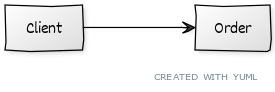
\includegraphics[width=0.6\linewidth]{images/SolidOcpViolationUml}
	\caption{Diagram UML, gdzie \texttt{Client} narusza zasadę OCP.}
	\label{lab1/fig/SolidOcpViolationUml}
\end{figure}
%[Client]->[Order]
%[Client]
%[Order]

Stosując wzorzec projektowy strategia, który zostanie omówiony na kolejnych zajęciach mamy możliwość odwrócenia zależności. Jeśli w~wyniku rozszerzania, zmian funkcjonalności okaże się, że klasa \texttt{Order} powinna zostać zamieniona, będzie można utworzyć nową wersję klasy implementującej interfejs zdefiniowany przez klienta i ją podmienić bez modyfikacji w samej klasie \texttt{Client}.

%Zastosowano interfejs IClient zamiast IOrder, ponieważ związki klas abstrakcyjnych z klasami klienckimi są ściślejsze niż z konkretnymi potomnymi, które je implementują.
\begin{figure}[hbt!]
	\centering
	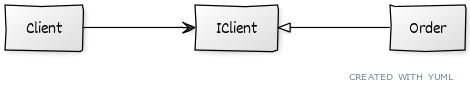
\includegraphics[width=0.9\linewidth]{images/SolidOcpUml}
	\caption{Diagram UML, gdzie \texttt{Client} \textbf{nie} narusza zasady OCP.}
	\label{lab1/fig/SolidOcpUml}
\end{figure}
%[Client]->[IClient]^[Order]
%[Client]
%[IClient]
%[Order]

Wyobraźmy sobie moduł odpowiedzialny za rysowanie figur geometrycznych. Parametrem jednej z~jego metod (\texttt{DrawerShape}) jest kolekcja obiektów. Jeśli w wyniku zmian konieczne okaże się dodanie nowej klasy np. \texttt{Diamond} wymagane będą zmiany w klasie \texttt{Drawer}.
\begin{lstlisting}[caption={Naruszenie zasady OCP}, label={lab1/lst/ocpViolationShapes}]
public class Circle { }
public class Square { }

public static class Drawer 
{
	public static void DrawShapes(IEnumerable<object> shapes) 
	{
		foreach (object shape in shapes) 
		{
			if (shape is Circle) 
			{
				(shape as Circle).DrawCircle();
			} 
			else if (shape is Square) 
			{
				(shape as Square).DrawSquare();
			}
		}
	}
}
\end{lstlisting}

Stosując polimorfizm i abstrakcję możemy uniezależnić klasę \texttt{Drawer} od konkretnych typów. Dzięki utworzeniu wspólnego interfejsu i przekazywanie listy obiektów implementujących ten interfejs, dodanie nowej figury nie będzie wymagało zmian w kodzie klienta. Nie musimy dostosowywać już istniejące kodu do zmian.

\begin{lstlisting}[caption={Poprawne zastosowanie zasady OCP}, label={lab1/lst/ocpShapesCorrect}]
public interface IShape 
{ 
	void Draw(); 
}
public class Circle : IShape { public void Draw() { }}
public class Square : IShape { public void Draw() { } }

public static class Drawer 
{
	public static void DrawShapes(IEnumerable<IShape> shapes) 
	{
		foreach (IShape shape in shapes) 
		{
			shape.Draw();
		}
	}
}
\end{lstlisting}

%Niestety istnieją takie zmiany, na które powyżej pokazana implementacja nie jest odporna np. jeśli kolejność rysowania figur okazałaby się konieczna do uwzględnienia. To projektant musi przewidzieć jakie zmiany są najbardziej prawdopodobne i określić odpowiednie zabezpieczenia. Zamiast stosować punkty szczepień (miejsca w programie, w których przewidujemy, że być może kiedyś będą zmiany), może zastosować zasadę mówiącą, że "Gdy raz mnie oszukasz, powinieneś się wstydzić. Kiedy oszukasz mnie po raz drugi, to ja powinienem się wstydzić". Jednocześnie powinniśmy na bieżąco sprawdzać nasze oprogramowanie i zdobywać wiedzę o prawdopodobnych rodzajach zmian. 

%Problem z kolejnością rysowanych figur możnaby rozwiązać stosując dodatkową klasę ShapeComparer : IComparer, która to zawiera statyczną tablicę priorytetów, na której to podstawie określane są priorytety rysowania figur. Metoda DrawShapes może wtedy wywolać metodę shapes.Sort(new ShapeComparer) prze rysowaniem figur (str. 186).

Oczywiście zmiany będą również konieczne w module, który tworzy instancje obiektów typu \texttt{Shape}. Ale ten proces jest zazwyczaj hermetyzowany w metodzie \texttt{Main} albo w fabrykach\ref{sec/lab2/abstractFactory}.

\subsubsection{Zadanie 2}
Utwórz nowy projekt i dodaj do niego klasę o~nazwie \texttt{UI} z metodą \texttt{Drawer} analogicznie jak zostało to pokazane powyżej\ref{lab1/lst/ocpShapesCorrect}. Utwórz w osobnych plikach klasy: \texttt{Circle}, \texttt{Square}, \texttt{Rectangle} oraz \texttt{Triangle}. Wszystkie powinny implementować interfejs \texttt{IShape} posiadający metodę \texttt{Draw()}. Zaimplementuj w klasach kształtów ten interfejs przez proste wypisywanie na ekranie konsoli informacji, że funkcja \texttt{Draw} została wywołana na przykład w następujący sposób:
\begin{lstlisting}
public class Square : IShape
{
	public void Draw() => Console.WriteLine("Square has been drawn.");
}
\end{lstlisting}
W metodzie \texttt{Main} utwórz kilka instancji klas kształtów i dodaj je do listy albo innego kontenera mogącego przechowywać obiekty implementujące interfejs \texttt{IShape}. Następnie przekaż do metody \texttt{DrawShapes} tę listę (wcześniej utwórz obiekt klasy \texttt{Draw}, aby móc z niej skorzystać).

\subsection{LSP - Zasada podstawienia Liskov (ang. SO\textbf{L}ID)}

Zasada podstawienia Liskov pozawala odpowiedzieć na pytanie jakie są dobre praktyki tworzenia hierarchii klas i co zrobić, aby były one zgodne z zasadą otwarte-zamknięte. Klient powinien móc bez zastanowienia się używać wymiennie klasy bazowej oraz klas pochodnych. W sytuacji braku możliwości podstawienia obiektów pochodnych w miejsce obiektów klasy bazowej występuje naruszenie zasady LSP. Często w konsekwencji zostaje również naruszona zasada OCP.

\begin{myboxWithTitle}{Zasada podstawienia Liskov}
Musi istnieć możliwość zastępowania typów bazowych ich podtypami.
\end{myboxWithTitle}

Lepsze zrozumienie zasady LSP można uzyskać analizując popularny przykład klasy prostokąta oraz klasy kwadratu, która jest pochodną klasy prostokąta. Zasadność stosowania dziedziczenia często jest analizowania przez zadanie sobie pytania czy klasy są w relacji \textbf{IS-A}. Niewątpliwie kwadrat jest prostokątem. Jednak pierwszy problem pojawia się w~sytuacji, gdy chcemy zaimplementować/skorzystać z~właściwości \texttt{Height} i~\texttt{Width} oraz dalej metody \texttt{Area}, zwracającej pole powierzchni danej figury. Właściwości \texttt{Height} i~\texttt{Width} są całkowicie uzasadnione w~przypadku prostokąta, jednak wątpliwe w klasie kwadratu. 

Próbując rozwiązać ten problem można próbować napisać klasę \texttt{Square} tak, że w momencie ustawiania właściwości wysokości albo szerokość w klasie kwadratu, będzie ustawiana zarówno wysokości jak i szerokość na taką samą wartość. Właściwości te mogą w klasie bazowej być wirtualne. Spójrzmy na poniższy kod, w~sytuacji gdy do funkcji zostałby przekazany właśnie taki obiekt kwadratu.
\begin{lstlisting}[caption={Naruszenie zasady LSP}, label={lab1/lst/lspViolationSquareRectangle}]
void Foo(Rectangle r)
{
	r.Width = 5;
	r.Height = 4;
	if(r.Area() != 20) {throw new ...}
}
\end{lstlisting}

Pomimo tego zabiegu klient dalej nie jest w~stanie użyć instancji klasy pochodnej zamiennie w klasą bazową. Najlepszym rozwiązaniem byłoby pominięcie dziedziczenia i napisania klasy \texttt{Sqaure} tak, aby nie dziedziczyła ona po \texttt{Rectangle}.

Przewidzieć takie założenia, można za pomocą  programowanie przez kontrakt (tzw. DBC ang. Design By Contract). Polega ona na dodaniu do metod pewnych warunków wejściowych oraz wyjściowych, które muszą być spełnione, aby metoda mogła się wykonać. 

\begin{mybox}
Ponowna deklaracja procedury (w klasie potomnej) może zastępować warunki wstępne tylko warunkami równymi lub słabszymi, natomiast warunki wyjściowe może zastępować tylko warunkami równymi lub mocniejszymi.
\end{mybox}

Warunki wyjściowe właściwości \texttt{Rectangle.Width} mogłyby zostać zdefiniowane jako:
\begin{lstlisting}
	assert((width == w ) && (height == old.height));
\end{lstlisting}

Innym problemem, może być sytuacja, gdy dana metoda klasy bazowej przyjmuje dowolny obiekt, natomiast w~klasie pochodnej istnieje nieznany wymóg, że obiekt ten musi być konkretnego typu np. z~powodu wykonywania operacji rzutowania. Klasa pochodna będzie zgłaszać niezrozumiały dla klienta wyjątek.

Reguły którymi należy się kierować, aby zachować zgodność z zasadą LSP mogą zostać podzielone na dwie kategorie: warunki kontraktu oraz warunki wariancji. Podczas laboratoriów skupimy się na tych pierwszych. Warunki wariancji natomiast są związane z zmiennością argumentów i typów zwracanych. 
%The concept of type variance in the languages of the Common Language Runtime (CLR) of the Microsoft .NET Framework is limited to generic types and delegates. However, variance in these scenarios is well worth exploring and will equip you with the requisite knowledge to write code that is LSP compliant for variance. This will be explored in depth in the “Covariance and contravariance” section later in this chapter

\subsubsection{Warunki kontraktu}
Warunki wstępne klasy bazowej nie mogą zostać zaostrzone w klasie pochodnej. Warunki końcowe nie mogą zostać złagodzone w klasie pochodnej. Inwarianty muszą pozostać takie same w klasie pochodnej jakie były w~klasie bazowej.

% Często zamienie mówi się, że programiści powinni programować do interfejsów oraz programować do kontraktu. Interfejsy jednak słabo przekazują informację o kontrakcie. Sygantury bardzo niewiele mówią o wymaganiach i gwarancji wywoływanej metody. W językach silnie typowanych jedyne co mamy to informację o typie, ale w tym miejscu intefejsy się kończą i w ich miejsce wchodzą kontrakty. 
% Bardzo wazne jest, aby nazwy argumentow byly opisowe, metody powinny od razu informować co robią, a argumenty czym są. Można nawet w nazwach dodac jednostki miar, aby dodatkowo sprezycoważ argument. 

Sygnatura określona w interfejsie danej metody informuje o tym jakiego typu parametry metoda przyjmuje. Jednak w przypadku, gdy wymagane są dodatkowe ograniczenia np. waga przedmiotu nie może być liczbą ujemną, konieczne jest użycie kontraktu. Warunki początkowe powinny być definiowane tak, aby metoda mogła się wykonać poprawnie. Jednym ze sposobów, aby wymusić stosowanie kontraktu jest rzucenie wyjątkiem, w~przypadku złej wartości argumentu wejściowego. Jeśli kontrakt nie zostanie spełniony, klient będzie zmuszony przechwycić i obsłużyć wyjątek, w przeciwnym razie wykonywanie programu się zakończy.

Warto w tym miejscu powiedzieć, że w przypadku kontraktów należy używać wyjątków, a nie asercji. Asercje służą, do znajdowania naszych błędów, natomiast wyjątki, aby poradzić sobie z błędami popełnionymi przez użytkowników czy innych programistów wykorzystujących nasz kod. Inaczej mówiąc, w przypadku sprawdzania warunków w~publicznym API należy stosować wyjątki. Jeśli sprawdzamy własne, wewnętrzne warunki można używać asercji.

Asercji można używać bardzo liberalnie. Informują one o tym czego kod oczekuje w danym momencie. Wyjątki dotyczą bardziej tego czego żądamy. Dobrze napisane asercje mogą nam powiedzieć nie tylko co się stało oraz gdzie, ale również dlaczego. Służą za dodatkową dokumentację. Jeśli podczas działania programu wystąpi błąd związany z asercją możemy dołączyć debugger do procesu i sprawdzić stan stosu. 
% Asercje z kodu produkcyjnego zostają wycięte może się wydawać, że stosowanie ich nie ma sensu. Jednak jeśli poźniej będzie konieczność odtworzenia problemu przez dewelopera to łatwo będzie możliwość znalezienia źródła problemu.

\subsubsection{Zadanie 3}

Stwórz nowy projekt .NET 5.0.



Utwórz klasę o nazwie \texttt{ShippingStrategy} i dodaj do niej metodę \texttt{CalculateShippingCost}, która będzie przyjmowała argumenty: \texttt{float packageWeigthInKilograms}, \texttt{float packageDimensionXInInches}, \texttt{float packageDimensionYInInches}, \texttt{RegionInfo destination}.

Na górze pliku \texttt{ShippingStrategy} dodaj przestrzeń nazw: \texttt{System.Globalization}, aby móc skorzystać z~\texttt{RegionInfo}:
\begin{lstlisting}
using System.Globalization;
//...
\end{lstlisting}

Wewnątrz metody utwórz zmienną pomocniczą typu \texttt{decimal} i przypisz do niej dowolną wartość (nie ma ona w tym momencie znaczenia). Będzie ona przechowywała zwracaną wartość, nadaj jej stosowną opisową nazwę.

Dodaj do metody kontrakt w postaci rzucanego wyjątku typu \texttt{ArgumentOutOfRangeException} w~przypadku, gdy przekazywane parametry są niewłaściwe np. są liczbami ujemnymi:
\begin{lstlisting}
public decimal CalculateShippingCost(float packageWeightInKilograms, float packageDimensionXInInches, float packageDimensionYInInches, RegionInfo destination)
{
	//Preconditions
	if (packageWeightInKilograms <= 0)
	{
		throw new ArgumentOutOfRangeException(nameof(packageWeightInKilograms), "Package weight can not be negative");
	}
	//...
}
\end{lstlisting}

Na końcu metody zwróć utworzoną wcześniej pomocniczą zmienną.

Analogicznie warunki końcowe powinny być sprawdzane na końcu metody, aby zagwarantować że metoda nie zmieniła stanu obiektu albo, że zwracana wartość jest poprawna. Dodaj warunek końcowy, który będzie sprawdzał, czy obliczone koszty wysyłki są dodatnie. W~przeciwnym razie zgłoś wyjątek.
\begin{lstlisting}
public decimal CalculateShippingCost(float packageWeightInKilograms, float packageDimensionXInInches, float packageDimensionYInInches, RegionInfo destination)
{
	//...
	//Postconditions
     if (shippingCost <= decimal.Zero) throw new ArgumentOutOfRangeException(nameof(shippingCost), "Shipping cost is out of range");
	
	return shippingCost;
}
\end{lstlisting}


W metodzie \texttt{Main} utwórz obiekt klasy \texttt{ShippingStrategy} i wywołaj funkcję z poprawnymi i~błędnymi argumentami, sprawdź czy został wygenerowany wyjątek.

Dodatkowo jeśli klient ma możliwość zmiany pewnej właściwości, która musi przyjmować ściśle określone wartości, powinna ona również zostać zabezpieczona w analogiczny sposób. Jeśli właściwość ta byłaby chroniona, albo prywatna, a jaj wartość byłaby ustawiana w konstruktorze, sprawdzenie należałoby dodać w~konstruktorze klasy.

W utworzonej przed chwilą klasie dodaj prywatną \textbf{zmienna} typu \texttt{decimal} o nazwie \texttt{flatRate}.

Dodaj właściwość \texttt{FlatRate} z metodą dostępu \texttt{get} oraz akcesorem \texttt{set}.

Wewnątrz akcesora \texttt{set} dodaj sprawdzenie ustawianej wartości tak jak dla warunków początkowych i końcowych.
\begin{lstlisting}
public class ShippingStrategy
{
	private decimal flatRate;
	public decimal FlatRate 
	{ 
		get { return flatRate;}
		set
		{
			//Data invariants
			if (value <= decimal.Zero) throw new ArgumentOutOfRangeException(nameof(value), "Flat rate must be positive and non zero");
			flatRate = value;
		}
	}
	//...
}
\end{lstlisting}
Sprawdź działanie powyższego kontraktu z poziomu klienta - metody \texttt{Main}.


Zamiast umieszczać kod kontraktów wewnątrz metody, lepiej byłoby utworzyć osobne klasy typu \texttt{Weight} czy \texttt{Size} i~to w~nich dodać powyższe kontrakty. Dodaj do projekt klasy pomocnicze \texttt{Size} oraz \texttt{Weight} w dwóch osobnych plikach:
\begin{lstlisting}
public class Size
{
	public double Height { get; init; }
	public double Width { get; init; }
	
	public Size(double height, double width)
	{
		this.Height = height;
		this.Width = width;
	}
}
\end{lstlisting}
\begin{lstlisting}
public class Weight
{
	public double Value { get; init; }
	
	public Weight(double value) => this.Value = value;
}
\end{lstlisting}

W~ten sposób w~całym kodzie kontrakty dla danych typów będą spójne oraz zmniejszy się liczba duplikowanego kodu. Utwórz nowe klasy \texttt{Weight} oraz \texttt{Size} i~umieść w nich właściwości wraz z~zabezpieczeniem przed możliwością ustawienia niepoprawnej wartości. Klasa \texttt{Weight} może posiadać właściwość \texttt{Value}, natomiast \texttt{Size} właściwości \texttt{Height}, \texttt{Width}. Zamień deklarację i ciało metody \texttt{CalculateShippingCost} tak, aby korzystała z~tych klas.

\subsubsection{Zadanie 4}
Zbadaj kontrakty w kontekście zasady LSP:

Oznacz metodę \texttt{CalculateShippingCost} jako wirtualną. Utwórz klasę pochodną względem \texttt{ShippingStrategy} i nazwij ją np. \texttt{WorldWideShippingStrategy}. Za pomocą słowa kluczowego \texttt{override} przesłoń wirtualną metodę klasy bazowej i~dodaj w~niej sprawdzenie czy wartość argumentu \texttt{destination} jest \texttt{null}. Warunek ten narusza zasadę LSP mówiącą o tym, że nie wolno zaostrzać warunków początkowych. %dotyczy argumentu destination
\begin{lstlisting}
public class WorldWideShippingStrategy : ShippingStrategy
{	
	public override decimal CalculateShippingCost(Weight packageWeightInKilograms, Size packageDimensionInInches, RegionInfo destination)
	{
		//LSP violation
		if (destination == null) throw new ArgumentNullException(nameof(destination), "Destination can not be null or empty");
		//...
	}
}
\end{lstlisting}

Utwórz teraz w metodzie \texttt{Main()} dwa obiekty w sposób pokazany poniżej\ref{lab1/lst/lspShippingStrategiesCall}. 

Zwróć uwagę, że w drugim przypadku został zgłoszony wyjątek. Klient musi w takiej sytuacji rozróżniać różne typu wykorzystywanych obiektów co łamie zasadę LSP oraz wprowadza dodatkowe zależności.  

\begin{lstlisting}[caption={Wywołanie metod klas ShippingStrategy oraz WolrdWideShippingStrategy}, label={lab1/lst/lspShippingStrategiesCall}]
class Program
{
	static void Main(string[] args)
	{
		ShippingStrategy shippingStrategyCustom = new ShippingStrategy();
		ShippingStrategy shippingStrategyWorldWide = new WorldWideShippingStrategy();
		
		var retA = shippingStrategyCustom.CalculateShippingCost(new Weight(10),  new Size(10, 10), null);
		var retB = shippingStrategyWorldWide.CalculateShippingCost(new Weight(10), new Size(10, 10), null);
	}
}
\end{lstlisting}

Analogicznie złamany może być warunek końcowy. Załóżmy, że w klasie bazowej \texttt{ShippingStrategy} tak jak wcześniej koszt wysyłki zawsze jest niezerowy. Natomiast w klasie pochodnej może on być zerowy jeśli, wysyłka jest do tego samego kraju: %dotyczy zmiennej shippingCost
\begin{lstlisting}
public class WorldWideShippingStrategy : ShippingStrategy
{	
	public override decimal CalculateShippingCost(Weight packageWeightInKilograms, Size packageDimensionInInches, RegionInfo destination)
	{
		//...
		//Postconditions LSP violation 
		if (destination == RegionInfo.CurrentRegion)
		{
			shippingCost = decimal.Zero;
		}
	}
}
\end{lstlisting}

Powoduje to ponowne złamanie zasady, że warunki końcowe nie powinny być rozluźniane w klasie pochodnej. Dokładnie ta sama zasada dotyczy wartości niezmiennych (ang. invariant data). W~naszym przykładzie właściwości \texttt{FlatRate}. Klasa pochodna nie powinna w żaden sposób zmieniać nałożonych wcześniej ograniczeń. Aby to sprawdzić dodaj do klasy \texttt{WorldWideShippingStrategy} ponownie właściwość wraz ze słowem kluczowym \texttt{new}:
\begin{lstlisting}
public class WorldWideShippingStrategy : ShippingStrategy
{
	//LSP violation
	public new decimal FlatRate { get; set; }
	//...
}
\end{lstlisting}

Sprawdź powyższe złamania zasady LSP w metodzie \texttt{Main}:
\begin{lstlisting}
class Program
{
	static void Main(string[] args)
	{
		var retC = shippingStrategyWorldWide.CalculateShippingCost(new Weight(10), new Size(10, 10), RegionInfo.CurrentRegion);
		(shippingStrategyWorldWide as WorldWideShippingStrategy).FlatRate = -20;
	}
}
\end{lstlisting}

Aby uprościć tworzenie kontraktów można napisać prostą metodę statyczną, która ułatwi ten proces:
\begin{lstlisting}
public class CustomContract
{
	public static void Requires<TException>( bool Predicate, string Message )
	where TException : Exception, new()
	{
		if ( !Predicate )
		{
			Debug.WriteLine( Message );
			throw new TException();
		}
	}
}  	
\end{lstlisting}

\texttt{Requires} jest metodą generyczną, gdzie \texttt{T} musi być typu referencyjnego oraz posiadać bezparametrowy konstruktor.

% Sytuacja może być niebezpieczne np. jeśli klient przez poczynione założenie, że wartość jest dodania wykona operację dzielenia przez zero.

%\subsubsection{Wykorzystanie kontraktów z \texttt{System.Diagnostics.Contracts}}

%Kontrakty z \texttt{System.Diagnostics.Contracts} nie są już wspierane.

%Jak można było zauważyć pisanie kontraktów w sposób pokazany powyżej może być żmudne. Dodatkowo sprawdzenie naruszenia kontraktu miało miejsce podczas wykonywania się programu. Wykorzystując kontrakty znajdujące się w przestrzeni nazw \texttt{System.Diagnostics.Contracts} można uprościć sobie proces tworzenia kontraktów.
%
%\begin{enumerate}
%	\item Utwórz nowy plik z klasą \texttt{ShippingStrategyCodeContracts}.
%	\item Dodaj na górze pliku przestrzeń nazw za pomocą \texttt{using System.Diagnostics.Contracts}.
%	\item Zamiast wykorzystywać klauzulę \texttt{if} utwórz kontrakt tak jak pokazano poniżej\ref{lab1/lst/lspCodeContractsPreCondition}. Zwróć uwagę, na odwróconą logikę wewnątrz metody \texttt{Requires} względem wcześniejszego przykładu. Dodatkowo istnieje możliwość zdefiniowana zgłaszanego wyjątku.
%	\item Analogicznie można utworzyć kontrakty dla warunków końcowych\ref{lab1/lst/lspCodeContractsPostCondition} oraz danych inwariantnych\ref{lab1/lst/lspCodeContractsDataInvariant}.
%\end{enumerate}

%\begin{lstlisting}[caption={Tworzenie kontraktów z wykorzystaniem \texttt{System.Diagnostics.Contracts} - warunki początkowe}, label={lab1/lst/lspCodeContractsPreCondition}]
%public class ShippingStrategyCodeContracts
%{
%	public virtual decimal CalculateShippingCost(float packageWeightInKilograms, float packageDimensionInInches, string destination)
%	{
%		//Preconditions
%		Contract.Requires(packageWeightInKilograms > 0);
%		Contract.Requires<ArgumentOutOfRangeException>(packageDimensionInInches > 0);
%		
%		//...
%	}
%}
%\end{lstlisting}

%\begin{lstlisting}[caption={Tworzenie kontraktów z wykorzystaniem \texttt{System.Diagnostics.Contracts} - warunki końcowe}, label={lab1/lst/lspCodeContractsPostCondition}]
%public class ShippingStrategyCodeContracts
%{
%	public virtual decimal CalculateShippingCost(float packageWeightInKilograms, float packageDimensionInInches, string destination)
%	{
%		//...
%		
%		//Postconditions
%		Contract.Ensures(Contract.Result<decimal>() > 0);
%		
%		return decimal.MinValue;
%	}
%}
%\end{lstlisting}

%\begin{lstlisting}[caption={Tworzenie kontraktów z wykorzystaniem \texttt{System.Diagnostics.Contracts} - dane inwariantne}, label={lab1/lst/lspCodeContractsDataInvariant}]
%public class ShippingStrategyCodeContracts
%{
%	[ContractInvariantMethod]
%	private void ClassInvariant()
%	{
%		Contract.Invariant(this.FlatRate > 0m, "Flat rate must be positive and non-zero");
%	}   
%	
%	public decimal FlatRate { get; set; }
%}
%\end{lstlisting}
\subsection{ISP - Zasada segregacji interfejsów (ang. SOL\textbf{I}D)}

Interfejsy klas nie powinny być rozbudowane/złożone. Jeżeli jedna klasa korzysta jedynie z~pewnych funkcjonalności jakie zakłada interfejs, a druga z innych to taki interfejs powinien zostać podzielony na dwa niezależne od siebie. Do celów zapewnienia zgodności z zasadą separacji interfejsów można skorzystać z~techniki dziedziczenia wielokrotnego. Należy pamiętać, że w C\# klasa nie może dziedziczyć po więcej niż jeden klasie, natomiast może implementować wiele interfejsów. Obiekty klienckie mogą korzystać z tego samego obiektu za pośrednictwem różnych interfejsów. Powinny one zależeć wyłącznie od wywoływanych przez siebie metod.  

\begin{myboxWithTitle}{Zasada segregacji interfejsów}
Klient nie powinien być zmuszany do zależności od metod, których nie używa.
\end{myboxWithTitle}

Wyobraźmy sobie, że musimy przygotować program obsługujący interfejs użytkownika bankomatu. Konieczne jest zapewnienie możliwości obsługi urządzenia z~wykorzystaniem interfejsu graficznego, syntezatora mowy oraz za pomocą języka Braille'a (klasy interfejsu użytkownika). 

Zakładamy, że każda oęperacja dowolnej transakcji jest realizowana przez osobną klas na przykład mogą to być typy: \texttt{DepositTransaction}, \texttt{WithdrowalTransaction} oraz \texttt{TransferTransaction}, wszystkie mogą dziedziczyć po abstrakcyjnej klasie bazowej \texttt{Transaction} z~pojedynczą metodą \texttt{Execute}. Jednocześnie wszystkie muszą korzystać z klas, które realizują funkcję UI (klasy te powinny implementować interfejs \texttt{IUI}). Klasa realizująca obsługę z wykorzystaniem syntezatora mowy, musi implementować wszystkie możliwe operacje przewidziane przez klasy pochodne względem \texttt{Transaction}, co jest sensowne. Problemem jest jednak fakt, że np. klasa \texttt{DepositTransaction} musi niepotrzebnie znać/posiadać referencje do całego obiektu implementującego UI. Wystarczyłaby by funkcja \texttt{RequestDepositAmount}, obiekt nie jest zainteresowany np. \texttt{RequestTransferAmount}. 

Rozwiązanie tego problemu zostało pokazano na diagramie UML~\ref{lab1/fig/SolidIspUml}. Dzieląc gruby interfejs \texttt{IUI} można odciążyć klientów od posiadania referencji do obiektów, których funkcjonalności nie potrzebują. Co więcej, jeśli zostanie dodana nowa transakcja np. \texttt{PayGasBillTransaction} nie będzie konieczności ponownej przebudowy pozostałych klas transakcji w~wyniku zmiany grubego interfejsu UI. 

\begin{figure}[hbt!]
	\centering
	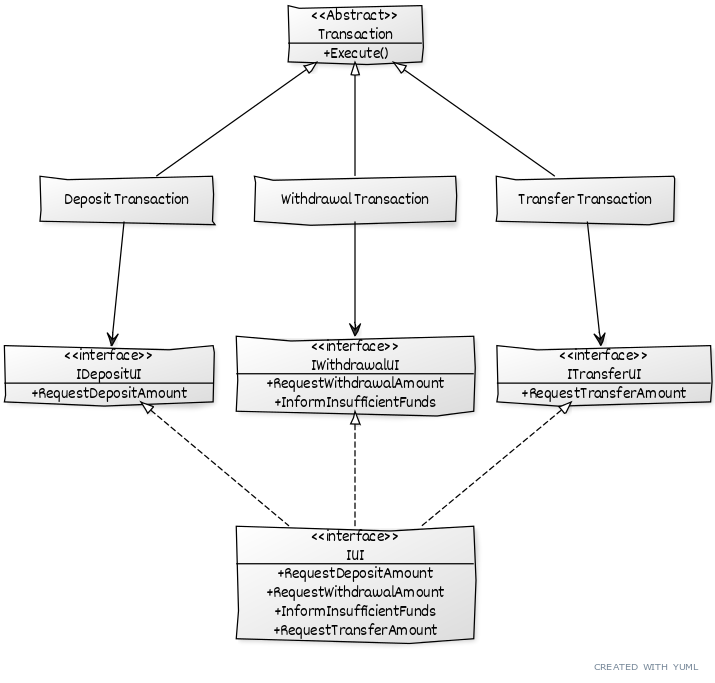
\includegraphics[width=0.8\linewidth]{images/SolidIspUml}
	\caption{Diagram UML projektu w którym zrealizowano zasadę segregacji interfejsów.}
	\label{lab1/fig/SolidIspUml}
\end{figure}
%[Transaction]^[Deposit Transaction]
%[Transaction]^[Withdrawal Transaction]
%[Transaction]^[Transfer Transaction]
%
%[Deposit Transaction]->[DepositUI]
%[Withdrawal Transaction]->[WithdrawalUI]
%[Transfer Transaction]->[TransferUI]
%
%[DepositUI]^-.-[UI]
%[WithdrawalUI]^-.-[UI]
%[TransferUI]^-.-[UI]
%
%[<<Abstract>>Transaction|+Execute()]
%
%[Deposit Transaction]
%[Withdrawal Transaction]
%[Transfer Transaction]
%
%[≪interface≫;DepositUI|+RequestDepositAmount]
%[≪interface≫;WithdrawalUI|+RequestWithdrawalAmount;+InformInsufficientFunds]
%[≪interface≫;TransferUI|+RequestTransferAmount]
%
%[≪interface≫;UI|+RequestDepositAmount;+RequestWithdrawalAmount;+InformInsufficientFunds;+RequestTransferAmount]

W sytuacji, gdy pewna klasa kliencka albo metoda, potrzebowałaby wykorzystać obiekt implementujący zarówno \texttt{IDepositUI} oraz \texttt{IWithdrowalUI}, można jako argumenty konstruktora albo metody przekazać dwa razy ten sam obiekt w następujący sposób: \texttt{Foo(ui,ui)}. Deklaracja konstruktora miałaby postać: \texttt{void Foo(IDepositUI depositUI, IWithdrowalUI withdrowalUi)}.

Ciekawym przykładem zastosowania zasady ISP jest wykorzystanie interfejsów do umożliwienia wykonywania operacji jedynie po wcześniejszym uwierzytelnieniu użytkownika. Przed operacją logowania klient korzysta z~interfejsu \texttt{IUnauthorized}:
\begin{lstlisting}
public interface IUnauthorized
{
	IAuthorized Login(string username, string password);
	void RequestPasswordReminder(string emailAddress);
}
\end{lstlisting}
natomiast po zalogowaniu, poprawnym uwierzytelnieniu, zwracany jest obiekt implementujący \texttt{IAuthorized}:
\begin{lstlisting}
public interface IAuthorized
{
	void ChangePassword(string oldPassword, string newPassword);
	void AddToBasket(Guid itemID);
	void Checkout();
	void Logout();
}
\end{lstlisting}
Drugi z wymienionych interfejsów umożliwia wykonanie większej liczby operacji. Rozwiązanie to zabezpiecza programistę przez udostępnieniem uprzywilejowanych operacji przez niezalogowanego użytkownika. Jest to lepsze rozwiązanie niż umieszczać w interfejsie wszystkie operacje jakie może użytkownik wykonać. 

\subsubsection{Zadanie 5}
Poniższy interfejs\ref{lab1/lst/ispCrudInterface} zawiera zbiór zapytań i poleceń do pamięci trwałej. Dalej natomiast została pokazana przykładowa implementacja\ref{lab1/lst/ispCrudInterfaceImplementation} tego interfejsu korzystająca z bazy danych MongoDB\footnote{Baza danych typu NoSQL w której dane przechowywane są jako pliki z formacie JSON.} do zapytań oraz NHibernate\footnote{Biblioteka ORM przeznaczone na platformę .NET do mapowania obiektów modelu domeny na relacyjną bazę danych.} do poleceń.
\begin{lstlisting}[caption={Interfejs zawierający zbiór operacji CRUD}, label={lab1/lst/ispCrudInterface}]
public interface IPersistence
{
	IEnumerable<Entity> GetAll();
	Item GetByID(Guid identity);
	IEnumerable<Entity> FindByCriteria(string criteria);
	void Save(Entity entity);
	void Delete(Entity entity);
}
\end{lstlisting}

\begin{lstlisting}[caption={Implementacja interfejsu \texttt{IPersistence}}, label={lab1/lst/ispCrudInterfaceImplementation}]
public class Persistence : IPersistence
{
	private readonly ISession session;
	private readonly MongoDatabase mongo;
	public Persistence(ISession session, MongoDatabase mongo)
	{
		this.session = session;
		this.mongo = mongo;
	}
	public IEnumerable<Entity> GetAll()
	{
		return mongo.GetCollection<Entity>("entities").FindAll();
	}
	public Entity GetByID(Guid identity)
	{
		return mongo.GetCollection<Entity>
		("entities").FindOneById(identity.ToBson());
	}
	public IEnumerable<Entity> FindByCriteria(string criteria)
	{
		var query = BsonSerializer.Deserialize<QueryDocument>
		(criteria);
		return mongo.GetCollection<Entity>("entities").Find(query);
	}
	public void Save(Entity entity)
	{
		using(var transaction = session.BeginTransaction())
		{
			session.Save(entity);
			transaction.Commit();
		}
	}
	public void Delete(Entity entity)
	{
		using(var transaction = session.BeginTransaction())
		{
			session.Delete(entity);
			transaction.Commit();
		}
	}
}
\end{lstlisting}
Często można natomiast się spotkać z rozdzieleniem operacji odczytu i aktualizacji bazy danych. Przykładem tej koncepcji jest m.in wzorzec CQRS, o którym szerzej będziemy mówić przy okazji czynnościowych wzorców projektowych~\ref{sec/lab4/cqrs}. Na ten moment najprościej ujmując polega on na rozdzieleniu operacji odczytu od operacji aktualizacji, dodawania i~usuwania z/do bazy danych.. 

Zastanów się jak można podzielić interfejs\ref{lab1/lst/ispCrudInterface} na dwa mniejsze: jeden dla poleceń, drugi dla zapytań. Dwie klasy np. \texttt{CommandsNHibernate} oraz \texttt{QueriesMongo} mogłyby implementować odpowiednio \texttt{ICommands} i~\texttt{IQueries}. Klasa kontrolera w takiej sytuacji mogłaby posiadać referencję do dwóch obiektów implementujących wspomniane interfejsy. Takie podejście pozwala na niezależne korzystanie z dwóch rodzajów baz danych, ich swobodną wymianę i skalowanie. Implementacje mogłyby znajdować się różnych w pakietach co jest dodatkową korzyścią 

Utwórz nowy projekt .NET 5.0 i~zaproponuj rozdzielenie powyższego interfejsu\ref{lab1/lst/ispCrudInterface} w~sposób wyżej opisany. Aby wyeliminować błędy kompilacji, konieczne będzie dodanie dwóch pakietów NuGet. W tym celu PPM kliknij na nazwę projektu i wybierz opcję Manage NuGet Packages. Następnie znajdź i zainstaluj pakiet \texttt{mongocsharpdriver} oraz \texttt{NHibernate}. Dodatkowo utwórz pustą klasę \texttt{Enitity}:
\begin{lstlisting}
public class Entity {}
\end{lstlisting}
%\begin{lstlisting}
%public interface IQueries
%{
%	IEnumerable<Item> GetAll();
%	Item GetByID(Guid identity);
%	IEnumerable<Item> FindByCriteria(string criteria);
%}
%// . . .
%public interface ICommands
%{
%	void Save(Item item);
%	void Delete(Item item);
%}
%\end{lstlisting}
%
%\begin{lstlisting}
%public class QueriesMongo : IQueries
%{
%	private readonly MongoDatabase mongo;
%	public QueriesMongo(MongoDatabase mongo) =>	this.mongo = mongo;
%	public IEnumerable<Item> GetAll()
%	{
%		return mongo.GetCollection<Item>("items").FindAll();
%	}
%	public Item GetByID(Guid identity)
%	{
%		return mongo.GetCollection<Item>
%		("items").FindOneById(identity.ToBson());
%	}
%	public IEnumerable<Item> FindByCriteria(string criteria)
%	{
%		var query = BsonSerializer.Deserialize<QueryDocument>
%		(criteria);
%		return mongo.GetCollection<Item>("Items").Find(query);
%	}
%}
%\end{lstlisting}
%
%\begin{lstlisting}
%public class CommandsNHibernate : ICommands
%{
%	private readonly ISession session;
%	public CommandsNHibernate(ISession session) => this.session = session;
%	public void Save(Item item)
%	{
%		using(var transaction = session.BeginTransaction())
%		{
%			session.Save(item);
%			transaction.Commit();
%		}
%	}
%	public void Delete(Item item)
%	{
%		using(var transaction = session.BeginTransaction())
%		{
%			session.Delete(item);
%			transaction.Commit();
%		}
%	}
%}
%\end{lstlisting}


\subsection{DIP - Zasada odwracania zależności (ang. SOLI\textbf{D})}

Głównie za sposób działania aplikacji odpowiadają moduły wysokopoziomowe. To one zawierają logikę biznesową, która często jest wielokrotnie wykorzystywana. Przemyślana architektura obiektowa powinna składać się z wyraźnie zdefiniowanych i odznaczających się warstw. Usługi powinny być opisane odpowiednimi, niezmiennymi interfejsami\footnote{Rzadko udaje się osiągnąć sytuację, w której interfejsy są niezmienne w szczególności na początkowym etapie projektu. Jednak powinny one być zdecydowanie bardziej stabilne niż klasy.}.

\begin{myboxWithTitle}{Zasada odwracania zależności}
	A. Moduły wysokopoziomowe nie powinny zależeć od modułów niskopoziomowych. Obie grupy modułów powinny zależeć od abstrakcji.\\
	B. Abstrakcje nie powinny zależeć od szczegółowych rozwiązań. To szczegółowe rozwiązania powinny zależeć od abstrakcji.
\end{myboxWithTitle}

Nie należy postrzegać bibliotek jako właścicieli interfejsów. Interfejsy powinny być powiązane ze swoimi właścicielami i to klasy z innej warstwy powinny implementować te interfejsy. % Lekki wstep o Clean Architecture Taylor'a i o tym jak interfejs opisujacy dostep do bazy danych znajduje sie w warstwie Application, natomiast implementacja w Infrastructure.
Pozwala to tworzyć oprogramowanie, które jest elastyczne. Jeśli dany zestaw jest wykorzystywany przez kilku klientów np. pobrany pakiet NuGet to warto stworzyć dodatkową warstwę abstrakcji, która umożliwi w~przyszłości zmianę tego pakietu, bez konieczności wprowadzania zmian po stronie klienta. Można to osiągnąć np. stosując wzorzec projektowy Adapter~\ref{sec/lab3/adapter}, który zostanie omówiony na przyszłych zajęciach. Oczywiście jeśli mamy do czynienia z klasami, które są zmieniane bardzo rzadko, albo mamy wysoki poziom zaufania to autorów to uzależnienie się od nich nie jest czymś złym. Ciężko znaleźć sens, tworzenia dodatkowej warstwy pośredniej do komunikowania się np. z~klasą \texttt{string}.

Wyobraźmy sobie przykład dwóch klas \texttt{Button} oraz \texttt{Lamp}. Klasa przycisku ma możliwość sterowania lampą. W~najprostszej, naiwnej implementacji można by dodać pole w klasie \texttt{Button} przechowujące referencje do obiektu lampy. \texttt{Lamp} mógłby być przekazywany np. jako argument konstruktora. Dlaczego te podejście jest złe i łamie zasadę DIP? \texttt{Button} będący wysokopoziomową abstrakcją, jest uzależniony od niskopoziomowego obiektu lampy.

Powyższy problem można rozwiązać przez dodanie interfejsu np. \texttt{ISwitchableDevice} i~wstrzykiwanie obiektu go implementującego do obiektu \texttt{Button}. Teraz wystarczy, aby \texttt{Lamp} implementował ten interfejs. W~przypadku, kiedy przycisk będzie miał zostać wykorzystany do sterowania np. silnikiem albo piecem wystarczy utworzyć nowy obiekt \texttt{Motor} albo \texttt{Heater}, który będzie implementował \texttt{ISwitchableDevice} i przekazać go do obiektu \texttt{Button}.

% Można narysować kilka warstw: Controllers, Services, Domain oraz NHibernate. Warstwy zależą od siebie w kolejności takiej jak zostały wymienione. Dodatkowo interfejsy przynależą do konkretnej warstwy np. w warstwie Services znajduje się SecurityService oraz ISecurityService. W tym przypadku jeśli skompilujemy np. Conrollers, dalej w katalogu /bin będzie najdował się NHibernate i inne warstwy.

Odpowiednim podejściem jest umieszczenie interfejsów oraz ich implementacji w osobnych zestawach. Klienci %klienci jako klasy, ktore korzystaja z obiektow innych klas, a nie metoda Main. Oczywiscie klasa/kontener IoC musi posiadac referencej, aby moc utworzy dane instancje.
powinny posiadać referencje jedynie do zestawu z interfejsem. W idealnym scenariuszu interfejsy nie powinny posiadać żadnych zależności, kod kliencki również. To implementacje powinny zależeć od interfejsów. 
\subsubsection{Zadanie 6}
Przeanalizuj poniższy kod i zmień go tak, aby był zgodny z omawianą zasadą DIP.
\begin{lstlisting}
public class Regulator
{
	const byte THERMOMETER = 0X86;
	const byte FURNACE = 0X87;
	const byte ENGAGE = 1;
	const byte DISENGAGE = 0;
	
	void Regulate(double minTemp, double maxTemp)
	{
		for (; ; )
		{
			while (this.Read(THERMOMETER) > minTemp)
			{
				Thread.Sleep(1000);
			}
			this.Write(FURNACE, ENGAGE);
			while (this.Read(THERMOMETER) < maxTemp)
			{
				Thread.Sleep(1000);
			}
			this.Write(FURNACE, DISENGAGE);
		}
	}
	
	byte Read(byte register)
	{
		return 0x00; //returned value not relevant.
	}
	void Write(byte register, byte value)
	{
		//...
	}
}
\end{lstlisting}
% engage - zalaczac, furnace - piec 
% In physics and materials science, the Curie temperature (TC), or Curie point, is the temperature above which certain materials lose their permanent magnetic properties. The Curie temperature is named after Pierre Curie, who showed that magnetism was lost at a critical temperature.[1]. Curie point electro-magnets have been proposed and tested for actuation mechanisms in passive safety systems of fast breeder reactors, where control rods are dropped into the reactor core if the actuation mechanism heats up beyond the material's curie point. Other uses include temperature control in soldering irons.

Możesz utworzyć dwa dodatkowe interfejsy, jeden dla obiektów mierzących temperaturę \texttt{ISensor} i drugi dla obiektów odpowiedzialnych za zmianę temperatury np. pieców \texttt{IDevice}. Dalej utwórz dwie klasy implementujące te interfejsy np. \texttt{Thermometer} oraz \texttt{Heater} i uzależnij obiekt regulacji od tych abstrakcji. Przekaż obiekt mierzący temperaturę oraz odpowiedzialny za sterownie urządzeniem przez konstruktor tej klasy. 

\subsection{Kontenery IoC (ang. Inversion of Control)}
Kontenery IoC takie jak Castle Windsor, Autofac czy Ninject ułatwiają wstrzykiwanie zależności. Jeśli pracujemy nad dużym projektem, w którym klasy zależą od wielu innych i wykorzystują mechanizm wstrzykiwania zależności można wykorzystać kontener IoC, aby ułatwić sobie proces tworzenia obiektów. 

Na przykład tworzenie obiektu \texttt{CustomerService} pokazanego poniżej\ref{lab1/lst/dpiComplexObjectConstruction} wymaga utworzeniu wielu innych obiektów i przekazania ich jako argumenty konstruktora.
\begin{lstlisting}[caption={Tworzenie obiektu posiadającego zależności wstrzykiwane przez konstruktor }, label={lab1/lst/dpiComplexObjectConstruction}]
public CustomerData GetCustomerData(string customerNumber)
{
	var customerApiEndpoint = ConfigurationManager.AppSettings["customerApi:customerApiEndpoint"];
	var logFilePath = ConfigurationManager.AppSettings["logwriter:logFilePath"];
	var authConnectionString = ConfigurationManager.ConnectionStrings["authorization"].ConnectionString;
	using(var logWriter = new LogWriter(logFilePath ))
	{
		using(var customerApiClient = new CustomerApiClient(customerApiEndpoint))
		{
			var customerService = new CustomerService(
			new SqlAuthorizationRepository(authorizationConnectionString, logWriter),
			new CustomerDataRepository(customerApiClient, logWriter),
			logWriter
			);   
			
			return customerService.GetCustomerData(string customerNumber);
		}
	}
}
\end{lstlisting}
Wykorzystując kontener IoC można zarejestrować zależności, które będą tworzone i wstrzykiwane automatycznie. Jeśli dana klasa potrzebuje np. obiektu implementującego \texttt{ILogWriter}, kontener utworzy odpowiednią instancję pod warunkiem, że została ona wcześniej zarejestrowana. Jeżeli np. tym obiektem jest \texttt{LogWriter} i wymaga on ścieżki do pliku, można również taką ścieżkę zarejestrować jako wartość klucza w~\texttt{AppSettings}. Kontener ,,wie'' jakie obiekty, jakich typów muszą być utworzone i wstrzyknięte, aby spełnić wymagania tworzonej klasy. Jeśli odpowiedni obiekt nie został wcześniej zarejestrowany to zostanie zgłoszony wyjątek o~tym informujący. Dodatkowo kontenery umożliwiają sprecyzowanie czy jedna i ta sama instancja ma zostać przekazana do wszystkich obiektów, które jej potrzebuje czy np. za każdym razem powinien być tworzony nowy obiekt.

Kontenery IoC powinny być wykorzystywane jedynie do wiązania poszczególnych elementów programu. Jeśli chcemy tworzyć obiekty podczas działania programu należy wykorzystywać fabryki. Trzeba unikać sytuacji w~których w~całym programie znajdują się referencje do kontenera. Zazwyczaj wystarcza jedno pobranie obiektu np. typu \texttt{Application}, natomiast reszta powiązań powinna odbywać się po stronie kontenera IoC.

\subsubsection{Zadanie 7}\label{lab1/ex/IoC}
Utwórz dwa projekty w solucji. Jeden niech będzie biblioteką, drugi natomiast aplikacją konsolową. Dodaj referencję do biblioteki w aplikacji konsolowej. Aby to zrobić kliknij PPM na projekt aplikacji konsolowej, dalej \texttt{Add} i \texttt{Project Reference...}, następnie wskaż odpowiedni zestaw. W~projekcie biblioteki utwórz następującą hierarchię klas pokazaną na rysunku\ref{lab1/fig/IoC}.
\begin{figure}[hbt!]
	\centering
	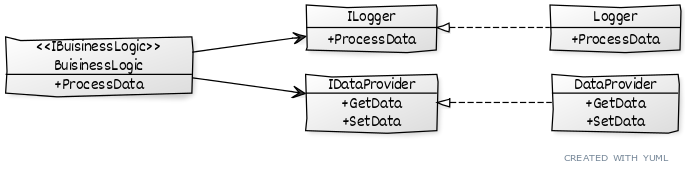
\includegraphics[width=0.8\linewidth]{images/ExerciseIocLib}
	\caption{Diagram UML hierarchii klas biblioteki z zadania~\ref{lab1/ex/IoC}}
	\label{lab1/fig/IoC}
\end{figure}

%[BuisinessLogic]->[ILogger]
%[BuisinessLogic]->[IDataProvider]
%[ILogger]^-.-[Logger]
%[IDataProvider]^-.-[DataProvider]
%
%[≪IBuisinessLogic≫;BuisinessLogic|+ProcessData]
%[ILogger|+ProcessData]
%[Logger|+ProcessData]
%[IDataProvider|+GetData;+SetData]
%[DataProvider|+GetData;+SetData]

Zaimplementuj metody tak, aby wypisywały informację na konsoli o tym jaka metoda jest aktualnie wykonywana np.:
\begin{lstlisting}
public class DataProvider : IDataProvider
{
	public void GetData() => Console.WriteLine("Loading the data");
	public void SetData() => Console.WriteLine("Saving the data");
}
\end{lstlisting}

Dodaj za pomocą menadżera pakietów NuGet pakiet \texttt{Autofac} do projektu aplikacji konsolowej.
Następnie utwórz w osobnym pliku klasę w której będzie następowała konfiguracja kontenera:
\begin{lstlisting}[caption={Konfiguracja kontenera IoC}, label={lab1/lst/autofacContainterConfig}]
public static class ContainerConfig
{
	public static IContainer Configure()
	{
		var builder = new ContainerBuilder();
		
		//...
		
		return builder.Build();
	}
}
\end{lstlisting}
Aby móc ,,pobrać'' instancję danej klasy z kontenera w pierwszej kolejności należy skojarzyć dane klasy z~odpowiadającymi im interfejsami. Inaczej mówiąc konieczne jest przekazanie informacji jaką klasę chcemy wykorzystać w miejsce danej abstrakcji. Należy to zrobić w następujący sposób:
\begin{lstlisting}
builder.RegisterType<BusinessLogic>().As<IBusinessLogic>();
//...
\end{lstlisting}
Powyższy fragment kodu oraz pozostałe rejestracje umieść w metodzie \texttt{Configure} klasy \texttt{ContainerConfig} \ref{lab1/lst/autofacContainterConfig}.

Do projektu aplikacji konsolowej dodaj również interfejs \texttt{IApplication}, z jedną metodą \texttt{Run()} nie zwracającą żadnego obiektu. W pliku \texttt{Application} umieść implementację interfejsu \texttt{IApplication}:
\begin{lstlisting}
public class Application : IApplication
{
	private readonly IBusinessLogic businessLogic;	
	public Application(IBusinessLogic businessLogic) => this.businessLogic = businessLogic;	
	public void Run() => businessLogic.ProcessData();
}
\end{lstlisting}

W metodzie \texttt{Main} umieść poniższy kod:
\begin{lstlisting}
static void Main(string[] args)
{
	//First thing we want to in program do is wireup the container and dependencies
	var container = ContainerConfig.Configure();
	
	using(var scope = container.BeginLifetimeScope()) //new scope 
	{
		var app = scope.Resolve<IApplication>(); //we need IApplication object, hence container gives us one
		app.Run();
	}
	
	Console.ReadLine();
}
\end{lstlisting}
Uruchom program i sprawdź, czy kontener poprawnie powiązał i stworzył wszystkie obiekty.

W momencie wywołania \texttt{Resolve} kontener sprawdza jakiego typu obiekty należy przekazać do konstruktora obiektu i wstrzykuje je za nas. W naszym przypadku po wywołaniu metody \texttt{Resolve<IApplication>} kontener ,,widzi'', że wymagany jest obiekt implementujący \texttt{IBusinessLogic}, aby utworzyć \texttt{Application}. Dalej \texttt{BusinessLogic} wymaga przekazania obiektu implementującego \texttt{ILogger} oraz \texttt{IDataProvider}. I~w~tym przypadku zostaną za nas utworzone odpowiednie obiekty i przekazane do \texttt{BusinessLogic} tak, aby mógł on zostać stworzony na potrzeby \texttt{Application}.

Aby ułatwić proces wiązania danych obiektów, można zamiast rejestrować poszczególne typy, zarejestrować cały zestaw wraz z określeniem pewnym warunków. Np. można zarejestrować wszystkie obiekty z~zestawu, których nazwy zaczynają się danym prefiksem, albo znajdują się w danym folderze. Można również powiązać wszystkie klasy z zestawu z odpowiadającymi im interfejsami.
\begin{lstlisting}
builder.RegisterAssemblyTypes(Assembly.Load(nameof(DependencyInversionPrincipleLib)))
//.Where(t => t.Namespace.Contains("Loggers")) //only from specific folder
.AsImplementedInterfaces(); //register the type as providing all of its public interfaces as services (excluding IDisposable).

\end{lstlisting}